\hypertarget{overview-of-project-progress}{%
\section{Overview of Project
Progress}\label{overview-of-project-progress}}

\emph{(Describe the overall team goals for the two weeks. These should
be an umbrella for the individual bi-weekly objectives, in prose)}

\hypertarget{achievements}{%
\subsection{Achievements}\label{achievements}}

\emph{(What were the main results from the two weeks. Documents, graphs,
working prototypes/ function. Team learning, bullet point)}

\begin{itemize}
\tightlist
\item
  example one
\item
  example two
\end{itemize}

\hypertarget{risks-issues-and-learning-points}{%
\subsection{Risks, Issues and Learning
Points}\label{risks-issues-and-learning-points}}

\emph{(What Problems have the team faced. How were these overcome? Is
support needed.)}

\begin{itemize}
\tightlist
\item
  example one
\item
  example two
\end{itemize}

\hypertarget{project-management-and-client-actions}{%
\section{Project Management and Client
Actions}\label{project-management-and-client-actions}}

\emph{(What admin tasks need completing. Any Actions that need flagging
up with the client)}

\begin{itemize}
\tightlist
\item
  example one
\item
  example two
\end{itemize}

\hypertarget{individual-work-packages}{%
\section{Individual Work Packages}\label{individual-work-packages}}

\hypertarget{alexander-charles}{%
\subsection{Alexander Charles}\label{alexander-charles}}

\hypertarget{objectives-and-tasks}{%
\subsubsection{Objectives and Tasks}\label{objectives-and-tasks}}

\emph{(What where you individual tasks for the two weeks. Any
outcomes?)}

\begin{itemize}
\tightlist
\item
  example one
\item
  example two
\end{itemize}

\hypertarget{knowledge-gained}{%
\subsubsection{Knowledge Gained}\label{knowledge-gained}}

\emph{(What did you learn? How have you/ will you use this learning to
help the project?)}

\begin{itemize}
\tightlist
\item
  example one
\item
  example two
\end{itemize}

\hypertarget{phoebe-staab}{%
\subsection{Phoebe Staab}\label{phoebe-staab}}

\hypertarget{objectives-and-tasks-1}{%
\subsubsection{Objectives and Tasks}\label{objectives-and-tasks-1}}

\begin{itemize}
\tightlist
\item
  example one
\item
  example two
\end{itemize}

\hypertarget{knowledge-gained-1}{%
\subsubsection{Knowledge Gained}\label{knowledge-gained-1}}

\begin{itemize}
\tightlist
\item
  example one
\item
  example two
\end{itemize}

\hypertarget{giovanni-tenderini}{%
\subsection{Giovanni Tenderini}\label{giovanni-tenderini}}

\hypertarget{objectives-and-tasks-2}{%
\subsubsection{Objectives and Tasks}\label{objectives-and-tasks-2}}

\begin{itemize}
\tightlist
\item
  example one
\item
  example two
\end{itemize}

\hypertarget{knowledge-gained-2}{%
\subsubsection{Knowledge Gained}\label{knowledge-gained-2}}

\begin{itemize}
\tightlist
\item
  example one
\item
  example two
\end{itemize}

\hypertarget{requirementss}{%
\section{Requirementss}\label{requirementss}}

\emph{(Describe the overall team goals for the two weeks. These should
be an umbrella for the individual bi-weekly objectives, in prose)}

\hypertarget{requirementss-1}{%
\section{Requirementss}\label{requirementss-1}}

\emph{(Describe the overall team goals for the two weeks. These should
be an umbrella for the individual bi-weekly objectives, in prose)}

\hypertarget{user-research}{%
\section{User Research}\label{user-research}}

this is some nice text bellow is an image.
\cite{blanchard2003macroeconomic}

\hypertarget{this-is-a-sub-heading}{%
\subsection{This is a sub heading}\label{this-is-a-sub-heading}}

\begin{figure}[H]
      \centering
      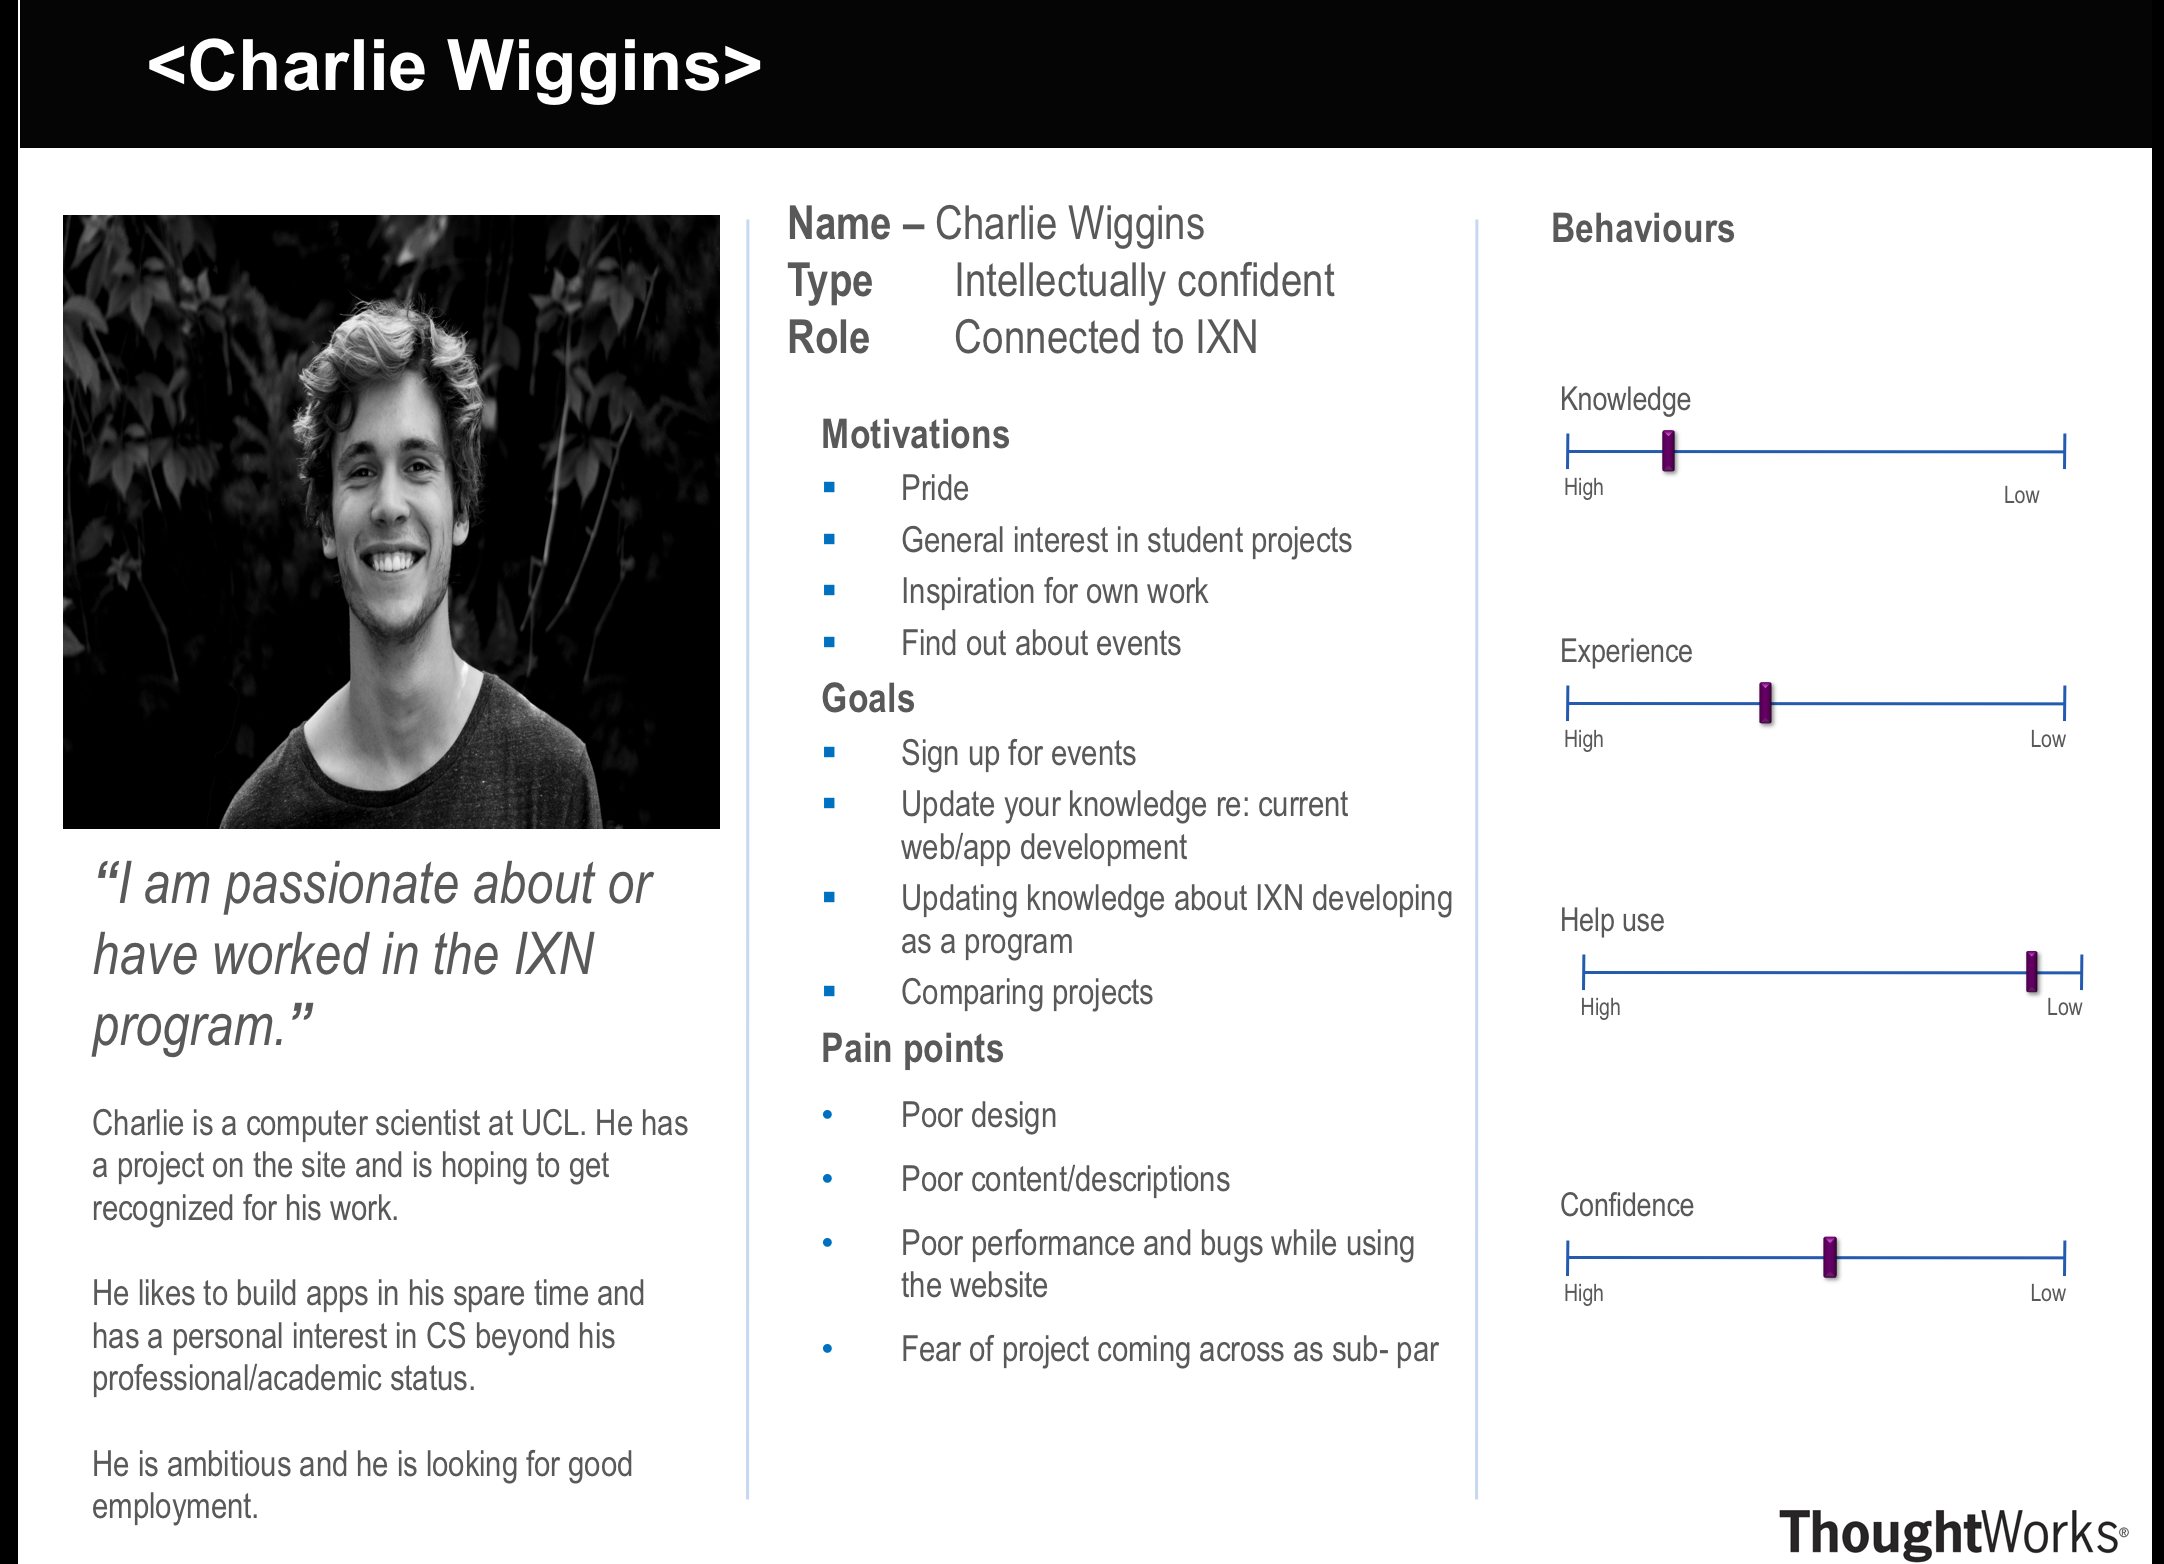
\includegraphics[trim = 0 0 0 0, clip, width=0.7\textwidth]{persona1.png}
      \caption{This is a persona}
      \label{persona1}
 \end{figure}

this image \cite{rumelt2012good} is of persona1 it is pretty good
\ref{persona1}

\newpage \# Requirementss \emph{(Describe the overall team goals for the
two weeks. These should be an umbrella for the individual bi-weekly
objectives, in prose)}

\hypertarget{requirementss-2}{%
\section{Requirementss}\label{requirementss-2}}

\emph{(Describe the overall team goals for the two weeks. These should
be an umbrella for the individual bi-weekly objectives, in prose)}

\hypertarget{requirementss-3}{%
\section{Requirementss}\label{requirementss-3}}

\emph{(Describe the overall team goals for the two weeks. These should
be an umbrella for the individual bi-weekly objectives, in prose)}

\hypertarget{requirementss-4}{%
\section{Requirementss}\label{requirementss-4}}

\emph{(Describe the overall team goals for the two weeks. These should
be an umbrella for the individual bi-weekly objectives, in prose)}

\hypertarget{requirementss-5}{%
\section{Requirementss}\label{requirementss-5}}

\emph{(Describe the overall team goals for the two weeks. These should
be an umbrella for the individual bi-weekly objectives, in prose)}

\section{Requirementss}\label{requirementss-1}

\emph{(Describe the overall team goals for the two weeks. These should
be an umbrella for the individual bi-weekly objectives, in prose)}

\section{Requirementss}\label{requirementss-2}

\emph{(Describe the overall team goals for the two weeks. These should
be an umbrella for the individual bi-weekly objectives, in prose)}

\section{Requirementss}\label{requirementss-3}

\emph{(Describe the overall team goals for the two weeks. These should
be an umbrella for the individual bi-weekly objectives, in prose)}

\section{Requirementss}\label{requirementss-4}

\emph{(Describe the overall team goals for the two weeks. These should
be an umbrella for the individual bi-weekly objectives, in prose)}

\section{Requirementss}\label{requirementss-5}

\emph{(Describe the overall team goals for the two weeks. These should
be an umbrella for the individual bi-weekly objectives, in prose)}

\section{Requirementss}\label{requirementss-6}

\emph{(Describe the overall team goals for the two weeks. These should
be an umbrella for the individual bi-weekly objectives, in prose)}

\section{Requirementss}\label{requirementss-7}

\emph{(Describe the overall team goals for the two weeks. These should
be an umbrella for the individual bi-weekly objectives, in prose)}
